\documentclass[9pt,a4paper]{extarticle}


	\usepackage[margin=5em,bottom=8em]{geometry}


%1 est la marge gauche
%2 est la marge en haut
%3 est la marge droite
%4 est la marge en bas
%5 fixe la hauteur de l'entête
%6 fixe la distance entre l'entête et le texte
%7 fixe la hauteur du pied de page
%8 fixe la distance entre le texte et le pied de page
%------------------------------Packages généraux------------------------------

\usepackage[english]{babel}
\usepackage[T1]{fontenc}
\usepackage{ae}
\usepackage[utf8]{inputenc}
\usepackage{scrextend}
\usepackage{hyperref}
 \hypersetup{
    colorlinks = true,
    linkcolor=black,
    urlcolor = black
    }
%-------------------------Mathématiques------------------------------
\usepackage{amsmath}
\usepackage{amssymb}
\usepackage{amsthm}
\usepackage{amsfonts}
\usepackage{eucal}
\newcommand\independent{\protect\mathpalette{\protect\independenT}{\perp}}
\def\independenT#1#2{\mathrel{\rlap{$#1#2$}\mkern2mu{#1#2}}}
%-----------------------Codes et algorithmes--------------------------
\usepackage{algorithm}
%\usepackage{algorithmic}
%\usepackage{clrscode3e}
\usepackage[noend]{algpseudocode}
%\newcommand{\pushline}{\Indp}% Indent
%\newcommand{\popline}{\Indm\dosemic}% Undent
%\newcommand{\nonl}{\renewcommand{\nl}{\let\nl\oldnl}}%


%------------------------------Graphics------------------------------

\usepackage{graphicx}
\usepackage{fancyhdr}
\usepackage{fancybox}
\usepackage{color}
\usepackage{pgf, tikz}
\usetikzlibrary{arrows, automata}
%\usepackage{slashbox}

%------------------Sub-sections--------%
\usepackage{titlesec}
\usepackage{hyperref}
\usepackage{comment}

\usepackage{hyperref}
               
 \hypersetup{
    colorlinks = true,
    linkcolor=black,
    urlcolor = black
    }
    
\newenvironment{solution}
    {%\begin{center}
    %\begin{tabular}{|p{0.9\textwidth}|}
    %\hline\\
    \color{red}
    }
    { 
    %\\\\\hline
    %\end{tabular} 
    %\end{center}
    \color{black}
    }
    
\newcommand{\blue}[1]{\textcolor{blue}{#1}}


\newif\ifhideproofs
%\hideproofstrue %uncomment to hide proofs

\ifhideproofs
\usepackage{environ}
\NewEnviron{hide}{}
\let\solution\hide
\let\endsolution\endhide
\fi

\title{{\bf INFO8006 Introduction to Artificial Intelligence}\\[1em]
Exercises 3: Games and adversarial search}
\date{}
%------------------------------Début du document------------------------------
\begin{document}
\maketitle
\vspace{-4em}
%------------------------------Page de garde------------------------------

  \section*{Learning outcomes}
    At the end of this exercise session you should be able to:
   \begin{itemize}
       \item Define formally the search problem associated to a game (IPATTU\footnote{Initial state - Player function - Actions function - Transition model - Terminal test - Utility function})
       \item Define and apply the Minimax algorithm
       \item Define and apply $\alpha-\beta$ pruning for Minimax
       \item Define H-Minimax, Expectiminimax, Monte-Carlo Tree Search
   \end{itemize}
   \section*{Exercise 1: Tic-Tac-Toe (AIMA, Ex 5.9)}
   \textit{Tic-tac-toe is a paper-and-pencil game for two players, X and O, who take turns marking the cells of a $3\times 3$ grid. The player who succeeds in placing three of their marks in a horizontal, vertical, or diagonal row wins the game.}\\
   We define $X_n$ as the number of rows, columns, or diagonals with exactly $n$ X's and no O's. Similarly, $O_n$ is the number of rows, columns, or diagonals
with just $n$ O's. The utility function assigns $+1$ to any position with $X_3 = 1$ and $-1$ to any
position with $O_3 = 1$. All other terminal positions have utility 0. For nonterminal positions,
we use a linear evaluation function defined as $Eval(s) = 3X_2(s)+X_1(s)-(3O_2(s)+O_1(s))$.\\
\begin{enumerate}
    \item Define the search problem associated with the Tic-tac-toe game.
    \begin{solution}
    \\
    Let us first define a game state $s \in \{-1, 0, 1\}^{3\times 3}$, where the three values $-1, 0, 1$ respectively denote O, empty and X cells.
    \begin{itemize}
        \item Initial state: $$ s_0 = 
        \begin{bmatrix}
        0 & 0 & 0\\
        0 & 0 & 0\\
        0 & 0 & 0
        \end{bmatrix}
        $$
        \item Player function:
        $
        player(s) = 1 \quad \text{if} \quad \Delta(s) = 0 \quad \text{and} \quad -1 \quad \text{otherwise}
        $, where $$\Delta(s) = \begin{bmatrix}1 & 1 & 1\end{bmatrix}s\begin{bmatrix}1 \\ 1 \\ 1\end{bmatrix}. $$
        \item Legal actions: An action is defined by a tuple $a = (a^1, a^2) \in \{0, 1, 2\}\times \{0, 1, 2\}$.
        $actions(s) = \{a : s_{a^1, a^2} = 0\}$.
        \item Transition model:
        $ result(s, a) = s' $ where $s'$ is the same as $s$ except that $s'_{a^1, a^2} = player(s)$.
        \item Terminal test:
        $terminal(s) = \text{True if } s \text{ contains 3 adjacent cells with +1, 3 adjacent cells with } -1\text{ or if the board is full}.$
        \item Utility function: $utility(s, p) = 1 \text{ if 3 adjacent cells with +1 else if the board is full }, 0 \text{ else} -1. $
    \end{itemize}
    \end{solution}
    \item Approximately how many possible games states of Tic-tac-toe are there?
    \begin{solution}
    \\
    If we disregard unreachable states, we have $3^{ 3 \times 3} = 19683$ possible states. And how many games (game state sequence)? $9! = 362880 $ 
    \end{solution}
    \item Show the whole game tree starting from an empty grid down to depth 2 (i.e., one X
and one O on the board), taking symmetry into account.
    \item Mark on your tree the evaluations of all the positions at depth 2.
    \item Using the minimax algorithm, mark on your tree the backed-up values for the     positions at depths 1 and 0, and use those values to choose the best starting move.
    \item Circle the nodes at depth 2 that would not be evaluated if $\alpha-\beta$ pruning were
applied, assuming the nodes are generated in the optimal order for $\alpha-\beta$ pruning.
\begin{solution}
See the figure below for the solutions to points 3 to 6.
\begin{center}
 
\includegraphics[width=.7\textwidth]{figures/tictactoe.pdf}   
\end{center}

\end{solution}
\end{enumerate}
\section*{Exercise 2: 21 misère game (January 2019)}
The game "21" is played as a misère game with any number of players who take turns saying a number. The first player says "1" and each player in turn increases the number by 1, 2, or 3, but may not exceed 21; the player who says "21" or a larger number   loses. 

\begin{enumerate}
    \item Define the search problem associated with the 2-player version of the "21" game.

    \begin{solution}
        We define a state $s$ as a pair $s = (s^0, s^1) \in \mathbb{Z}\times \{0, 1\}$ such that the first element $s^0$ is the value played by the last player and the second element $s^1$ corresponds to the player to play next. The first player has id $p=1$ and the second player has id $p=0$.
        \begin{itemize}
            \item Initial state: $s_0 := (s_0^0, s_0^1) := (1, 0)$.
            \item Player function: $player(\cdot): \mathbb{Z}\times \{0, 1\} \rightarrow \{0, 1\}$, such that
            $player(s= (s^0, s^1)) := s^1$.
            \item Action function: actions are denoted by the integer values that can be played by the current player. We define the action function $action(\cdot): \mathbb{Z}\times \{0, 1\}\rightarrow \mathbb{Z}^3$ such that $action(s= (s^0, s^1)) := \{s^0 + 1, s^0 + 2, s^0 + 3\} $.
            \item Transition function: $result(\cdot, \cdot): (\mathbb{Z}\times \{0, 1\})\times \mathbb{Z} \rightarrow \mathbb{Z}\times \{0, 1\}$ such that $result(s=(s^0, s^1), a) := (a, (s^1 + 1)\mod 2)$.
            \item Terminal function: $terminal(\cdot): \mathbb{Z}\times \{0, 1\} \rightarrow \{0, 1\}$ such that $terminal(s=(s^0, s^1)) := s^0 \geq 21$.
            \item Utility function: $utility(\cdot, \cdot): (\mathbb{Z}\times \{0, 1\}) \times \{0, 1\} \rightarrow \{-1, 1\}$ such that $utility(s=(s^0, s^1), p) := 1 - 2|p - s^0|$.
        \end{itemize}
    \end{solution}
    
    %\item Approximately how many possible games of "21" are there?
    \item For this subquestion and the following, consider the game of "5" (still in its 2-player version) which has the same rule except that you should not say 5 or more. Show the whole game tree.
    
    \begin{solution}
        \begin{figure}[h]
            \centering
            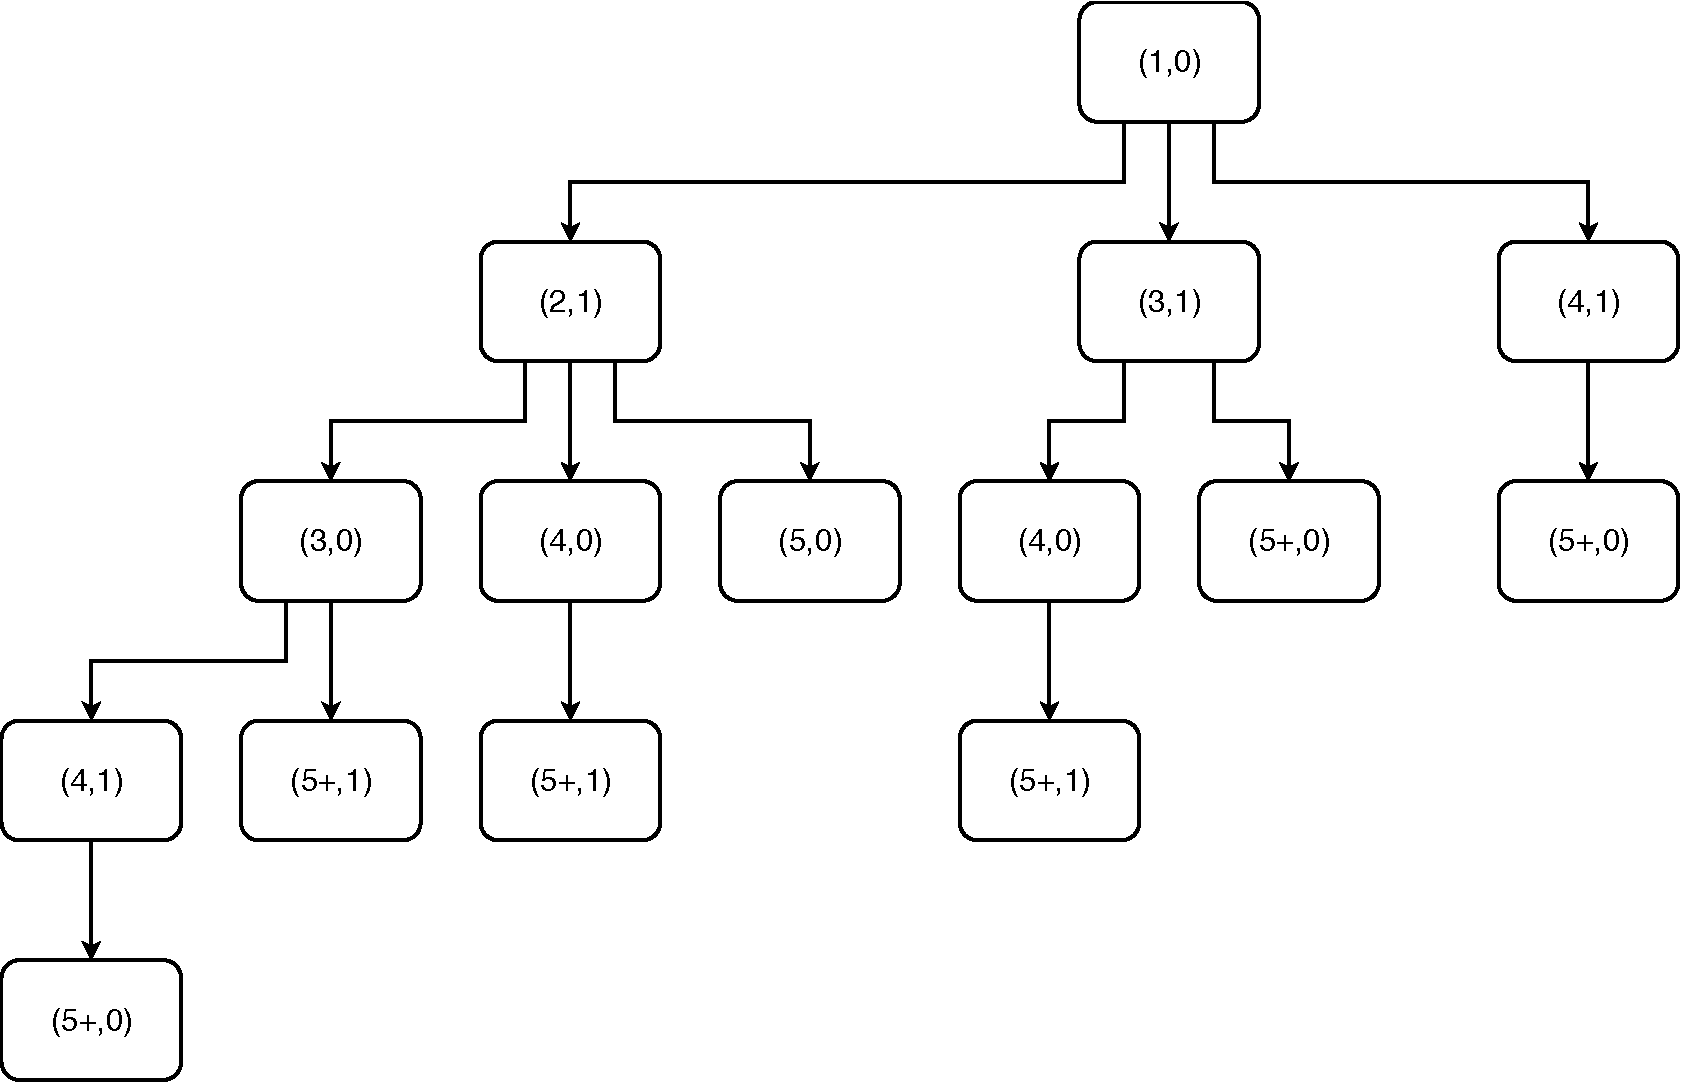
\includegraphics[width=.775\textwidth]{figures/tree_game.pdf}
            \label{fig:GT}
        \end{figure}
    \end{solution}
    
    \item \begin{enumerate}
        \item Using the minimax algorithm, mark on your tree the backed-up values, and use those values to choose the best starting move
        
        \begin{solution}
            From the game tree we conclude that the best move is to play $4$.
            NB: The winning strategy for the game of 21 is to always say a multiple of 4; it is then guaranteed that the other player will ultimately have to say "21" – so in the standard version where the first player opens with "1", they start with a losing move.
            \begin{figure}[h]
                \centering
                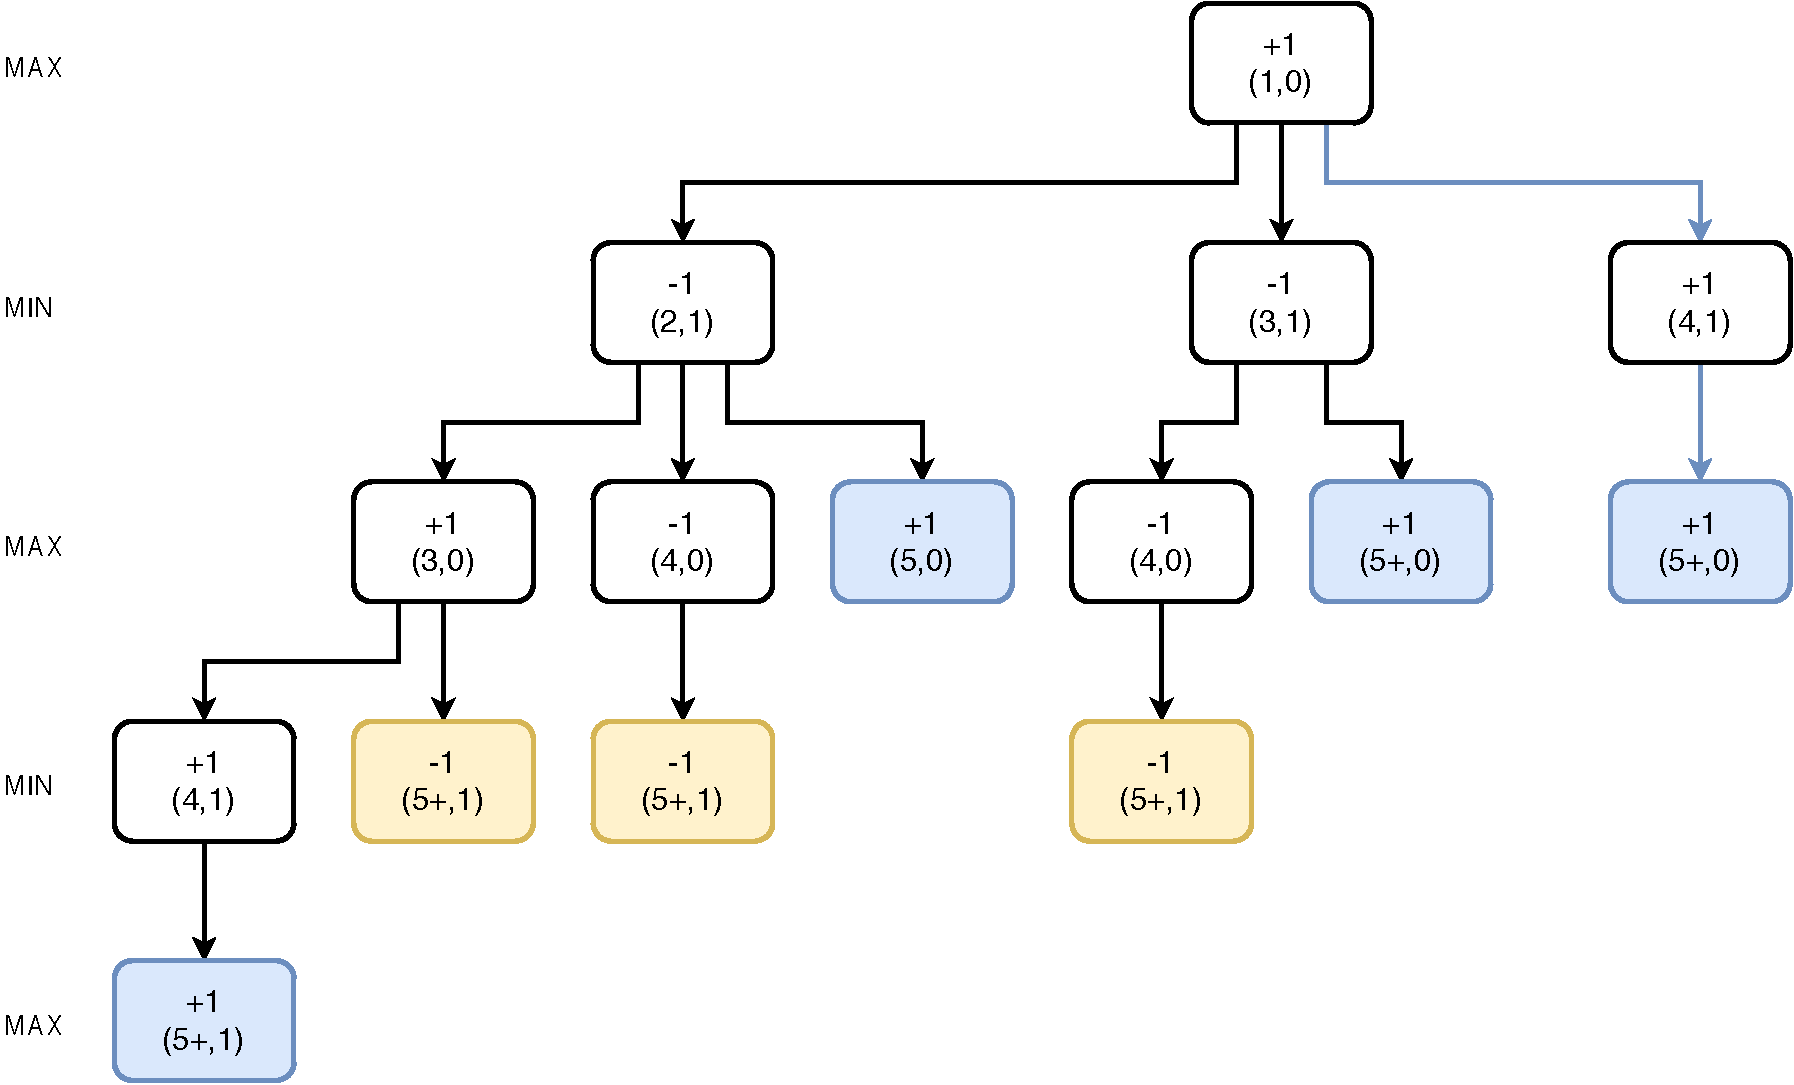
\includegraphics[width=.775\textwidth]{figures/tree_game_marked.pdf}
            \end{figure}
        \end{solution}
    
        \item Assume alpha–beta pruning were applied in optimal order. Draw the game tree containing only the nodes that would be evaluated.
        
        \begin{solution}
            Nodes that are not visited are colored in red.
            \begin{figure}[h]
                \centering
                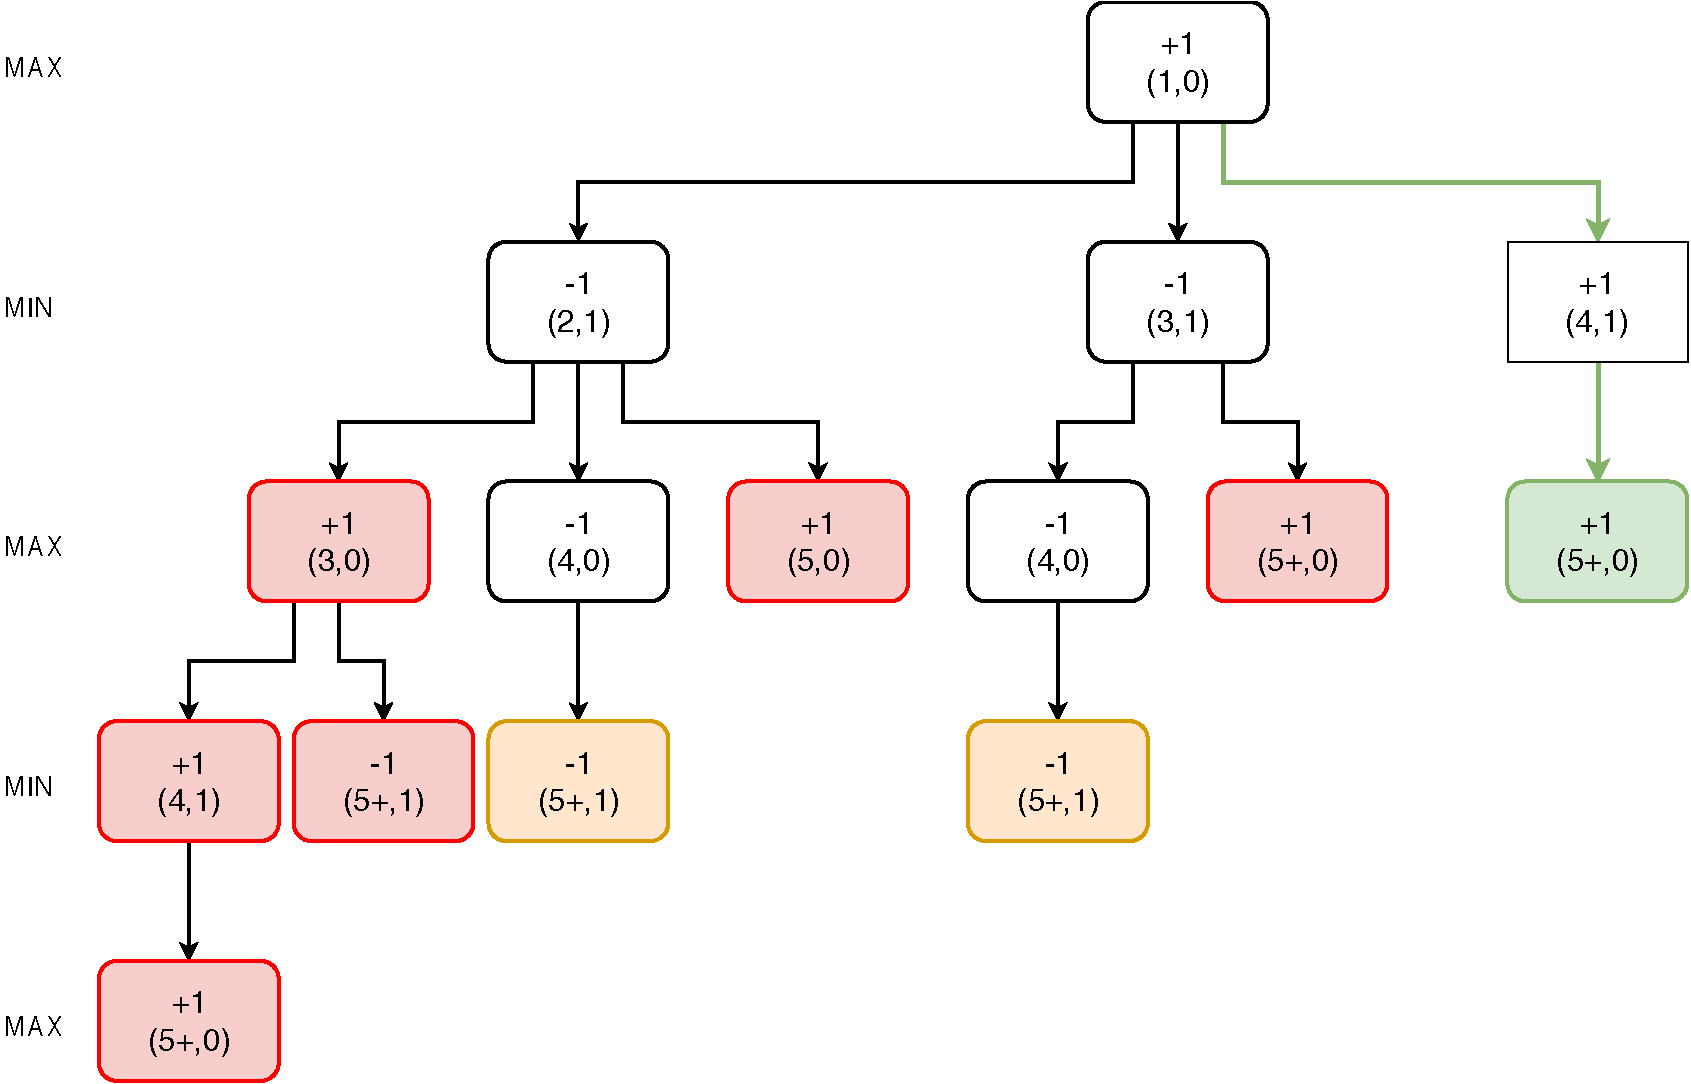
\includegraphics[width=.775\textwidth]{figures/alpha_beta_tree.pdf}
            \end{figure}
        \end{solution}
    \end{enumerate}
\end{enumerate}
   
\section*{Exercise 3: Quiz}
   \begin{enumerate}
       \item In a fully observable, turn-taking, zero-sum game between two perfectly rational players, it does not help the first player to know what strategy the second player is using (that is, what move the second player will make, given the first player’s move).
       \begin{solution}
       It doesn't help the 1st player to know the strategy of the other.
       \end{solution}
       \item What is a quiescent position?
       \begin{solution}
       A position in which the outcome of a game is unlikely to vary a lot in the near future.
       \end{solution}
       %\item What is the meaning of Q in the formula: $\frac{Q(n', p)}{N(n')} + c\sqrt{\frac{2\log N(n)}{N(n'}}$
       %\item What is the meaning of N in the formula: $\frac{Q(n', p)}{N(n')} + c\sqrt{\frac{2\log N(n)}{N(n'}}$
       \item In MCTS, what is encouraged by each term of the sum in the formula $\frac{Q(n', p)}{N(n')} + c\sqrt{\frac{2\log N(n)}{N(n'}}$?
       \begin{solution}
       1) Exploitation 2) Exploration.
       \end{solution}
       \item Which heuristic is correct (i.e. resulting in a rational agent) (see image below)?
       \begin{solution}
       Left.
       \end{solution}
   \end{enumerate}
   \begin{figure}[H]
       \centering
       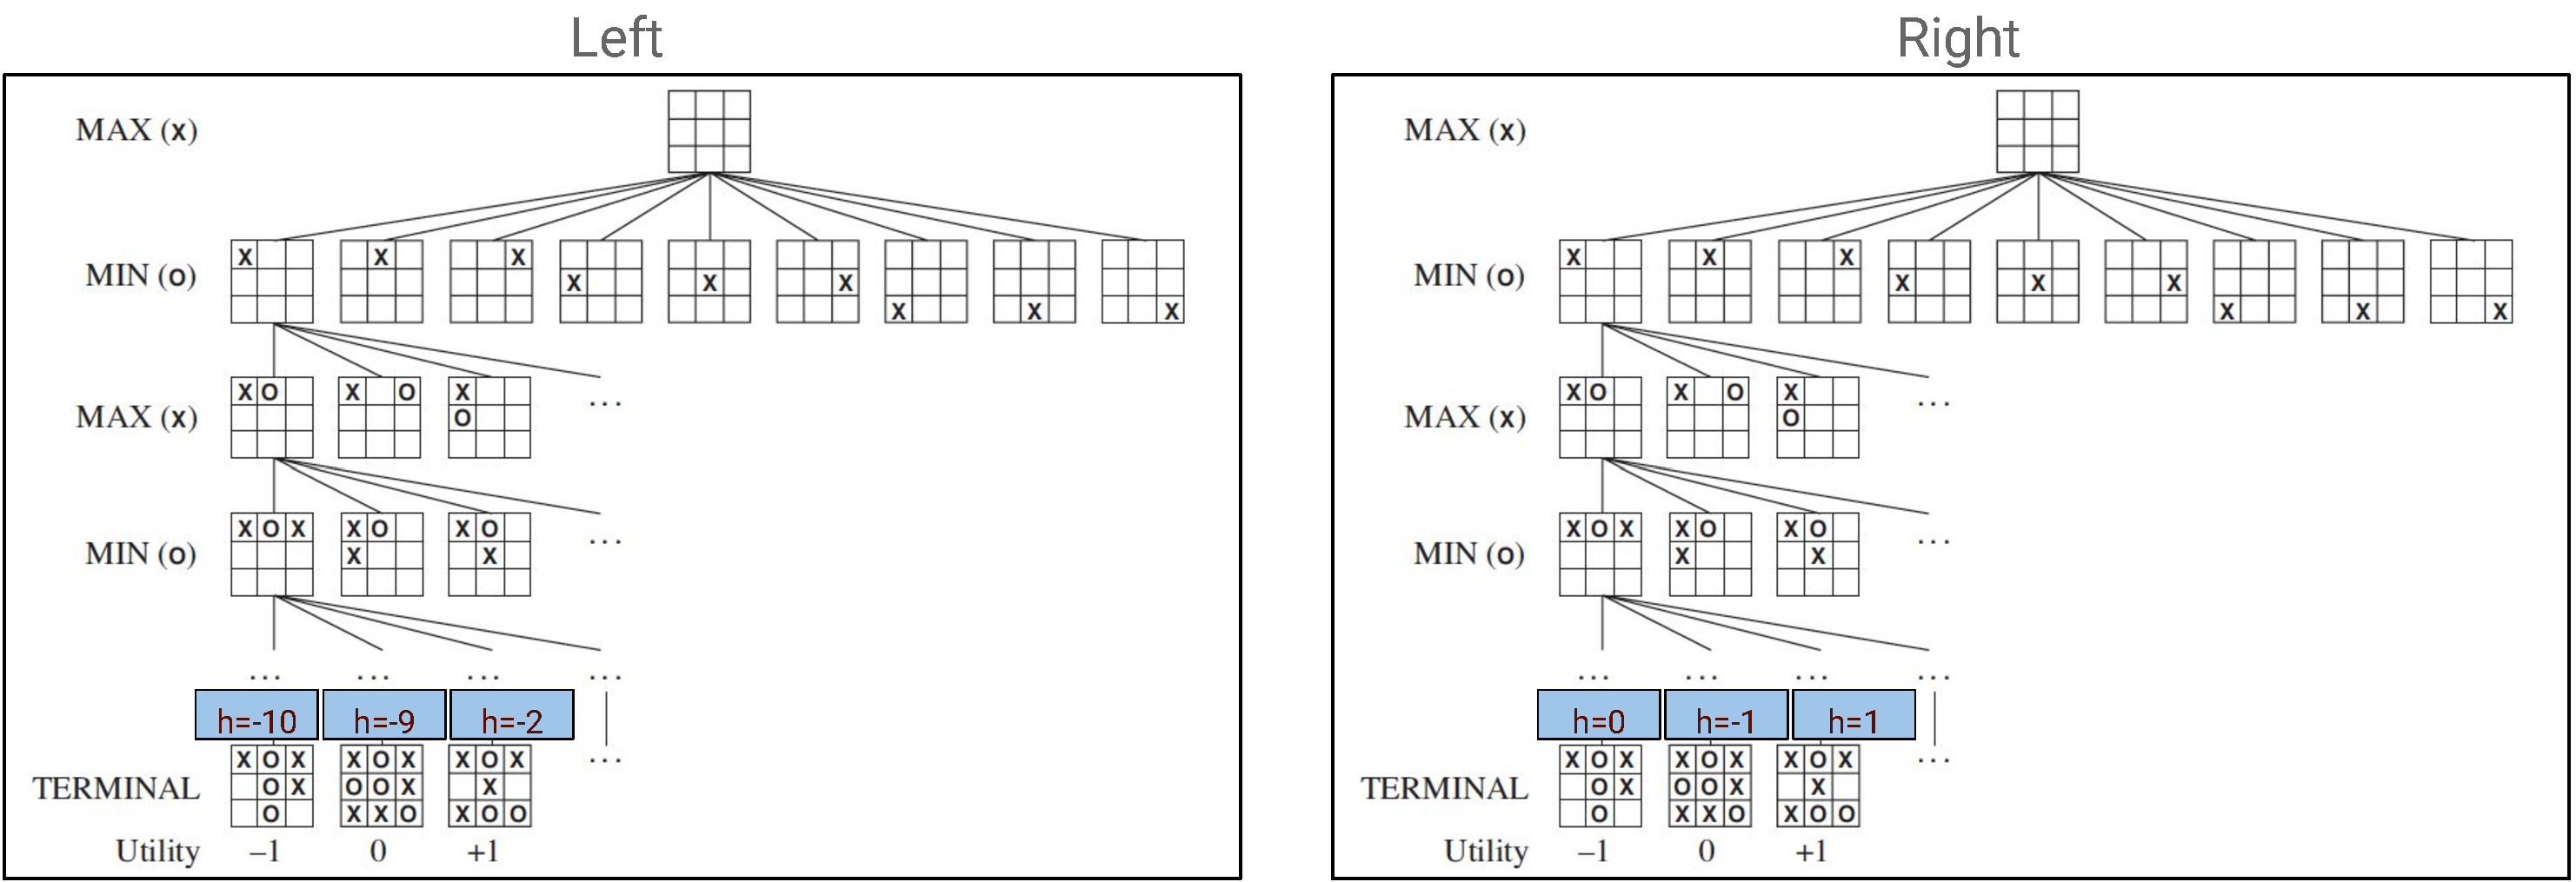
\includegraphics[width=1.\textwidth]{figures/trees.pdf}
       \caption{Two possible heuristics}
       \label{fig:my_label}
   \end{figure}
\section*{Exercise 4: Chess and transposition table $\star$ (AIMA, Ex 5.15)}
Suppose you have a chess program that can evaluate 16 million nodes per second.
Decide on a compact representation of a game state for storage in a transposition table.
\begin{enumerate}
    \item About how many entries can you fit in a 4-gigabyte in-memory table?
    \begin{solution}
    With 32 pieces, each needing 6 bits to specify its position on one of 64 squares, we need 24 bytes (6 32-bit words) to store a position, so we can store roughly 80 million positions in the table (ignoring pointers for hash table bucket lists).
    \end{solution}
    \item Will that be enough for the three minutes of search allocated for one move?
    \begin{solution}
    No, this is about 1/22 of the 1800 million positions generated during a three-minute search.
    \end{solution}
    \item How many table lookups can you do in the time it would take to do one evaluation? Suppose that you have a 3,2GHz machine and that it takes 20 operations to do one lookup on the transposition table.
    \begin{solution}
    The number of operations per evaluation is  $\frac{3.2\times 10^9 \text{op/s}}{16\times 10^6{eval/s}} = 200\text{op/eval}$, and so 10 lookups can be made for the same amount of time.
    \end{solution}
    %\item Now suppose the transposition table is stored on disk. About how many evaluations could you do in the time it takes to do one disk seek with standard disk hardware?
\end{enumerate}      
\section*{Exercise 5: Minimax $\star$ (Berkeley CS188 Fall 2019)}
\begin{center}
    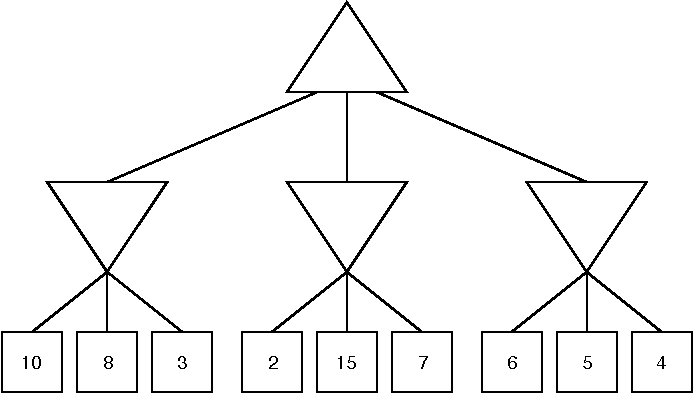
\includegraphics[width=.6\textwidth]{figures/minimax.pdf}
\end{center}
\begin{enumerate}
    \item Consider the zero-sum game tree shown above. Triangles that point up, such as at the top node (root), represent choices for the maximizing player; triangles that point down represent choices for the minimizing player. Assuming both players act optimally, fill in the minimax value of each node.
    \begin{solution}
    See the figure below.
    \begin{center}
        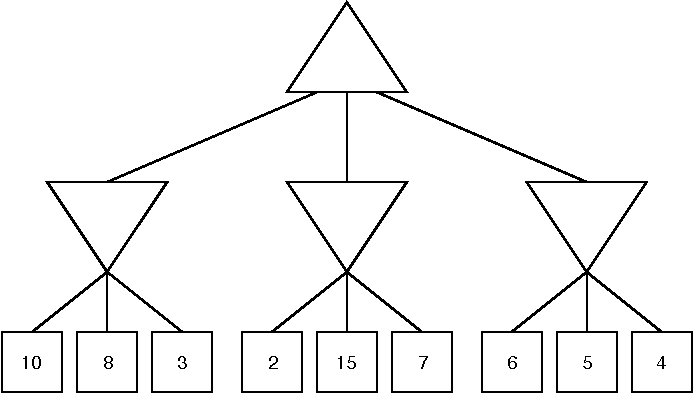
\includegraphics[width=.7\textwidth]{figures/minimax.pdf}
    \end{center}
    \end{solution}
    \item Which nodes can be pruned from the game tree above through alpha-beta pruning? If no nodes can be pruned, explain why not. Assume the search goes from left to right; when choosing which child to visit first, choose the left-most unvisited child.
    \begin{solution}
    See the figure below.
    \begin{center}
        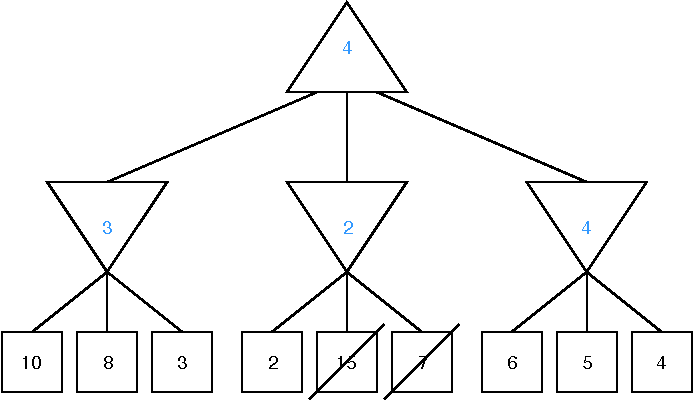
\includegraphics[width=.7\textwidth]{figures/minimax_sol_1.pdf}
    \end{center}
    \end{solution}
    \item  Again, consider the same zero-sum game tree, except that now, instead of a minimizing player, we have a chance node that will select one of the three values uniformly at random. Fill in the expectimax value of each node. The game tree is redrawn below for your convenience.
    \begin{solution}
    See the figure below.
    \begin{center}
        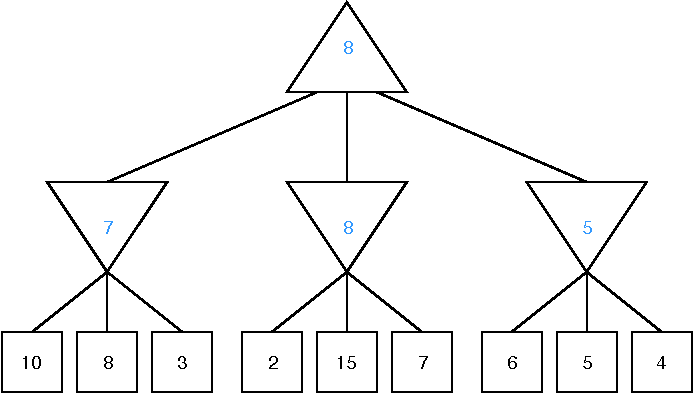
\includegraphics[width=.7\textwidth]{figures/minimax_sol_2.pdf}
    \end{center}
    \end{solution}
    \item Which nodes can be pruned from the game tree above through alpha-beta pruning? If no nodes can be pruned, explain why not.
    \begin{solution}
    No nodes can be pruned. There will always be the possibility that an as-yet-unvisited leaf of the current parent chance node will have a very high value, which increases the overall average value for that chance node. For example, when we see that leaf 4 has a value of 2, which is much less than the value of the left chance node, 7, at this point we cannot make any assumptions about how the value of the middle chance node will ultimately be more or less in value than the left chance node. As it turns out, the leaf 5 has a value of 15, which brings the expected value of the middle chance node to 8, which is greater than the value of the left chance node. In the case where there is an upper bound to the value of a leaf node, there is a possibility of pruning: suppose that an upper bound of +10 applies only to the children of the rightmost chance node. In this case, after seeing that leaf 7 has a value of 6 and leaf 8 has a value of 5, the best possible value that the rightmost chance node can take on is $\frac{6+5+10}{3} = 7$, which is less than 8, the value of the middle chance node. Therefore, it is possible to prune leaf 9 in this case.
    \end{solution}
\end{enumerate}
\end{document}
